% =====================================================================
% CAPÍTULO 4 — RESULTADOS
% ---------------------------------------------------------------------
% Pacotes: os mesmos do Capítulo 3 + \usepackage{graphicx} (figuras).
% Figuras: coloque a pasta "figuras/" (enviada junto) ao lado do .tex principal.
% Linhas marcadas com "% TODO" pedem conferência sua.
% Convenção: valores das tabelas com 4 casas decimais; no texto, arredondados.
% =====================================================================

\chapter{Resultados}
\label{cap:resultados}

Este capítulo apresenta os resultados obtidos com a metodologia descrita no Capítulo~\ref{cap:metodos}. Inicialmente, são apresentadas as principais características dos dados e o efeito da deduplicação. Em seguida, são reportados o desempenho dos quatro modelos no protocolo convencional de avaliação, a comparação estatística entre eles e seu custo computacional. Por fim, são apresentados os resultados dos experimentos complementares: a análise de importância de atributos, a avaliação com distribuição natural das classes, a avaliação em cenários não vistos durante o treino e o experimento de representação das portas. A interpretação conjunta desses resultados é feita no Capítulo~\ref{cap:discussao}.
% TODO: \label{cap:discussao} no capítulo de Discussão.

% ---------------------------------------------------------------------
\section{Caracterização dos dados e efeito da deduplicação}
\label{sec:res-dados}

A análise exploratória evidenciou diferenças marcantes entre as classes. Em relação ao protocolo, todas as classes maliciosas são compostas quase exclusivamente por conexões TCP, enquanto o tráfego benigno é majoritariamente UDP (cerca de 70\%), com aproximadamente 30\% de TCP e uma pequena parcela de ICMP. Em relação à duração, cerca de 94\% das conexões DDoS e dois terços das benignas têm duração nula ou ausente, ao passo que nenhuma conexão das classes Okiru e Attack apresenta essa característica. Entre as conexões com duração positiva, as conexões Okiru são as mais curtas, concentradas abaixo de um segundo. Essas diferenças sugerem que as classes são, em grande parte, separáveis a partir dos atributos do fluxo.

Como descrito na Seção~\ref{sec:dedup}, o IoT-23 apresenta um grau extremo de repetição de fluxos. A Tabela~\ref{tab:ablacao} apresenta o resultado do experimento de ablação, em que o RF binário foi avaliado com e sem as etapas de deduplicação.

\begin{table}[htbp]
\centering
\caption{Efeito da deduplicação sobre o RF binário.}
\label{tab:ablacao}
\begin{tabular}{lrr}
\toprule
\textbf{Condição} & \textbf{Teste repetido no treino (\%)} & \textbf{F1-macro} \\
\midrule
Sem nenhuma deduplicação         & 41,47 & 0,9981 \\
Sem a segunda deduplicação       &  0,21 & 0,9983 \\
Pipeline adotado (duas etapas)   &  0,00 & 0,9983 \\
\bottomrule
\end{tabular}
\\[2pt]
\small{Fonte: elaborado pelo autor.}
\end{table}

Sem nenhuma deduplicação, 41,5\% das amostras do conjunto de teste são idênticas a amostras do treino, ou seja, quase metade da avaliação seria feita sobre exemplos já vistos pelo modelo. A segunda deduplicação, por sua vez, elimina um vazamento residual de 0,2\%. Apesar disso, o F1-macro praticamente não se altera entre as condições. Esse resultado indica que a deduplicação é necessária para que a avaliação seja metodologicamente correta, mas que o alto desempenho do RF não é consequência do vazamento: dentro dos cenários estudados, as classes são de fato separáveis a partir dos atributos disponíveis.

% ---------------------------------------------------------------------
\section{Desempenho no protocolo convencional}
\label{sec:res-convencional}

A Tabela~\ref{tab:resultados-principais} apresenta o desempenho dos quatro modelos finais no conjunto de teste, com os hiperparâmetros selecionados na Seção~\ref{sec:hiperparametros} e ponderação de classes. A última coluna mostra a variabilidade do F1-macro: para RF, AD e SVM, a média e o desvio padrão da validação cruzada de 5 \textit{folds} no treino; para a CNN, a média e o desvio padrão das cinco execuções com sementes diferentes, avaliadas no teste. Os valores de teste da CNN correspondem à execução de F1 mediano.

\begin{table}[htbp]
\centering
\caption{Desempenho dos modelos finais no conjunto de teste (médias macro).}
\label{tab:resultados-principais}
\small
\setlength{\tabcolsep}{4pt}
\begin{tabular}{llrrrrc}
\toprule
\textbf{Tarefa} & \textbf{Modelo} & \textbf{Acurácia} & \textbf{Precisão} & \textbf{Recall} & \textbf{F1} & \textbf{F1 (repetições)} \\
\midrule
\multirow{4}{*}{Binária}
 & Árvore de Decisão & \textbf{0,9991} & \textbf{0,9990} & \textbf{0,9989} & \textbf{0,9990} & 0,9989 $\pm$ 0,0002 \\
 & Random Forest     & 0,9985 & 0,9982 & 0,9984 & 0,9983 & 0,9981 $\pm$ 0,0002 \\
 & CNN               & 0,9753 & 0,9636 & 0,9801 & 0,9713 & 0,9703 $\pm$ 0,0035 \\
 & SVM               & 0,9611 & 0,9434 & 0,9712 & 0,9554 & 0,9556 $\pm$ 0,0008 \\
\midrule
\multirow{4}{*}{Multiclasse}
 & Árvore de Decisão & \textbf{0,9989} & \textbf{0,9968} & \textbf{0,9977} & \textbf{0,9973} & 0,9971 $\pm$ 0,0017 \\
 & Random Forest     & 0,9986 & 0,9928 & 0,9974 & 0,9950 & 0,9933 $\pm$ 0,0031 \\
 & SVM               & 0,9226 & 0,7093 & 0,9235 & 0,7502 & 0,7505 $\pm$ 0,0048 \\
 & CNN               & 0,9029 & 0,6729 & 0,9140 & 0,7153 & 0,7370 $\pm$ 0,0482 \\
\bottomrule
\end{tabular}
\\[2pt]
\small{Fonte: elaborado pelo autor.}
\end{table}

Nas duas tarefas, os modelos baseados em árvores obtiveram desempenho praticamente perfeito, com F1-macro acima de 0,99, e a Árvore de Decisão superou ligeiramente o Random Forest. CNN e SVM ficaram em um patamar inferior: na tarefa binária, com F1-macro de 0,97 e 0,96, respectivamente; na multiclasse, com 0,72 e 0,75. A ordem entre esses dois modelos se inverte entre as tarefas, com a CNN à frente na binária e o SVM na multiclasse. Os resultados da validação cruzada e das repetições da CNN são consistentes com os de teste, o que indica que o desempenho observado não depende de uma partição particular dos dados.

Na tarefa binária, a diferença entre os grupos se deve principalmente a falsos positivos: o SVM classifica corretamente 99,65\% dos fluxos maliciosos, mas apenas 94,58\% dos benignos, o que reduz a precisão da classe maliciosa para 0,89. O mesmo padrão ocorre na CNN.

A Tabela~\ref{tab:f1-por-classe} detalha o F1 por classe na tarefa multiclasse. RF e AD superam 0,98 em todas as classes. Para SVM e CNN, as classes Attack, benigna, C\&C-HeartBeat e C\&C são bem reconhecidas, mas o desempenho cai acentuadamente em portscan, Okiru e, sobretudo, DDoS.

\begin{table}[htbp]
\centering
\caption{F1-Score por classe na tarefa multiclasse.}
\label{tab:f1-por-classe}
\begin{tabular}{lrrrrr}
\toprule
\textbf{Classe} & \textbf{Amostras (teste)} & \textbf{AD} & \textbf{RF} & \textbf{SVM} & \textbf{CNN} \\
\midrule
Benigno        & 36.986 & 0,9992 & 0,9990 & 0,9695 & 0,9628 \\
Portscan       &  5.990 & 0,9959 & 0,9950 & 0,7009 & 0,6198 \\
C\&C-HeartBeat &  4.706 & 1,0000 & 1,0000 & 0,9812 & 0,9794 \\
C\&C           &  3.248 & 0,9995 & 0,9991 & 0,8649 & 0,8336 \\
Attack         &  1.789 & 0,9997 & 0,9992 & 0,9870 & 0,9674 \\
Okiru          &    186 & 0,9866 & 0,9946 & 0,6525 & 0,5662 \\
DDoS           &     67 & 1,0000 & 0,9781 & 0,0957 & 0,0781 \\
\bottomrule
\end{tabular}
\\[2pt]
\small{Fonte: elaborado pelo autor.}
\end{table}

A Figura~\ref{fig:matrizes} mostra as matrizes de confusão do SVM e da CNN, normalizadas pela classe real. Os erros se concentram em dois pontos. O primeiro é a classe portscan: o SVM classifica 18\% desses fluxos como DDoS e 13\% como C\&C, e a CNN, 23\% e 17\%, respectivamente. O segundo é a classe benigna, da qual 4\% a 5\% dos fluxos são classificados como portscan. Embora esses percentuais pareçam modestos, eles se aplicam às classes mais numerosas do teste. Como resultado, mais de mil fluxos de portscan são previstos como DDoS, uma classe com apenas 67 amostras reais. É isso que reduz a precisão de DDoS para cerca de 0,05 nos dois modelos, apesar de um \textit{recall} próximo de 0,9. Raciocínio análogo explica a baixa precisão em Okiru (0,49 no SVM e 0,39 na CNN), causada por cerca de 200 a 300 fluxos benignos classificados nessa classe. RF e AD praticamente não cometem esses erros, e suas matrizes de confusão são quase diagonais.

\begin{figure}[htbp]
\centering
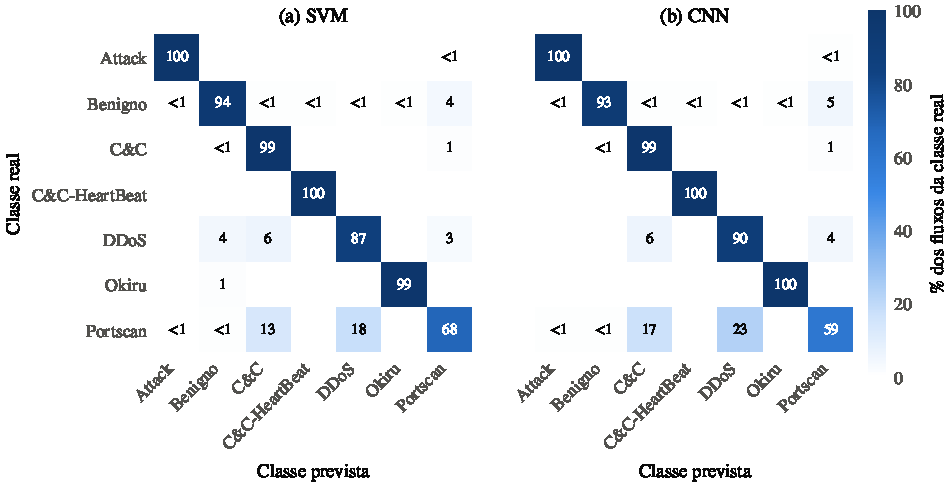
\includegraphics[width=\textwidth]{figuras/matrizes_svm_cnn_multiclasse.pdf}
\caption{Matrizes de confusão do SVM e da CNN na tarefa multiclasse, normalizadas pela classe real (\% dos fluxos de cada linha). Células vazias correspondem a zero.}
\label{fig:matrizes}
\par\vspace{2pt}
\small{Fonte: elaborado pelo autor.}
\end{figure}

\subsection{Efeito do balanceamento e do ajuste de hiperparâmetros}
\label{sec:res-ajuste}

Na tarefa binária, a substituição da ponderação de classes pelo SMOTE não trouxe ganho: o F1-macro do RF passou de 0,9983 para 0,9978, e o da AD, de 0,9990 para 0,9984. No SVM com hiperparâmetros padrão, o SMOTE elevou o F1-macro de 0,92 para 0,93, ao custo de mais que dobrar o tempo de treinamento (de 642 para 1.486~s). Esses resultados sustentam a adoção da ponderação de classes nos modelos finais.

O efeito do ajuste de hiperparâmetros variou conforme o modelo, como mostra a Tabela~\ref{tab:ajuste}. Para RF e AD, que já operavam próximos do limite superior com os valores padrão, o ganho na validação cruzada foi inferior a 0,0002. No SVM, o ajuste teve efeito expressivo. A primeira rodada melhorou a tarefa binária, mas piorou a multiclasse. Já a segunda rodada, com grade estendida e F1 ponderado pela prevalência real das classes, elevou o F1-macro de teste de 0,92 para 0,96 na tarefa binária e de 0,71 para 0,75 na multiclasse. Na CNN, a configuração padrão foi mantida na tarefa binária, e na multiclasse a busca selecionou uma configuração com \textit{dropout} maior e lote maior.

\begin{table}[htbp]
\centering
\caption{F1-macro no teste antes e depois do ajuste de hiperparâmetros.}
\label{tab:ajuste}
\begin{tabular}{llrr}
\toprule
\textbf{Modelo} & \textbf{Configuração} & \textbf{Binária} & \textbf{Multiclasse} \\
\midrule
RF  & padrão           & 0,9983 & 0,9951 \\
    & ajustado         & 0,9983 & 0,9950 \\
\midrule
AD  & padrão           & 0,9990 & 0,9973 \\
    & ajustado         & 0,9990 & 0,9973 \\
\midrule
SVM & padrão           & 0,9229 & 0,7055 \\
    & rodada 1         & 0,9418 & 0,6604 \\
    & rodada 2 (final) & 0,9554 & 0,7502 \\
\midrule
CNN & padrão (semente 42)               & 0,9735 & 0,6977 \\
    & final (média de 5 sementes)       & 0,9703 & 0,7370 \\
\bottomrule
\end{tabular}
\\[2pt]
\small{Fonte: elaborado pelo autor.}
\end{table}

As cinco execuções da CNN revelaram sensibilidade à semente aleatória na tarefa multiclasse: a execução com semente 42 alcançou F1-macro de 0,83, enquanto as outras quatro ficaram entre 0,70 e 0,72, o que explica o desvio padrão elevado (0,048). Essa mesma semente foi utilizada na busca aleatória, e a configuração selecionada se destacou das demais (F1 de 0,82 na validação, contra no máximo 0,72 das outras). Nas cinco execuções, porém, sua vantagem não se manteve. Isso indica que parte do resultado da busca refletiu a semente, e não a configuração. O uso da execução mediana nas comparações (Seção~\ref{sec:avaliacao}) protege a análise desse efeito. Na tarefa binária, as cinco execuções foram estáveis (F1 entre 0,964 e 0,974). A Figura~\ref{fig:curvas-cnn} mostra as curvas de treinamento da CNN multiclasse final: perda e acurácia de treino e de validação evoluem juntas, sem sinais de sobreajuste.

\begin{figure}[htbp]
\centering
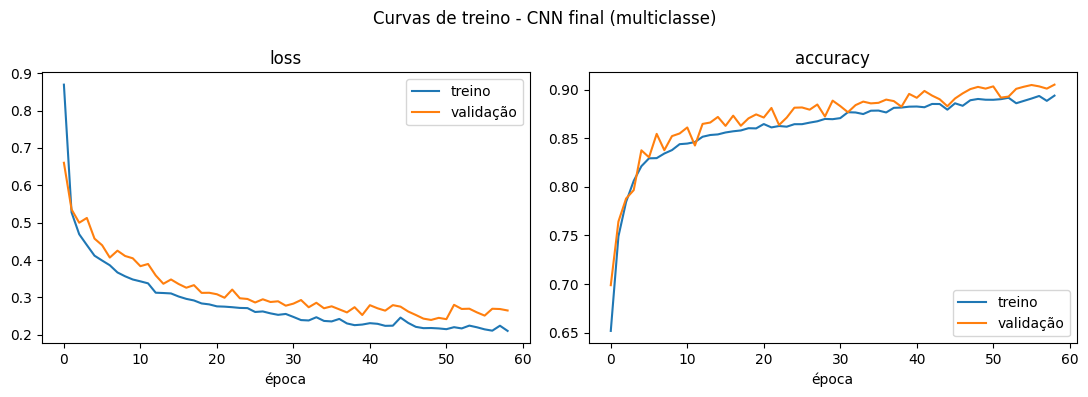
\includegraphics[width=0.9\textwidth]{figuras/curvas_cnn_multiclasse_final.png}
\caption{Curvas de perda (esquerda) e acurácia (direita) de treino e validação da CNN multiclasse final.}
\label{fig:curvas-cnn}
\par\vspace{2pt}
\small{Fonte: elaborado pelo autor.}
\end{figure}

% ---------------------------------------------------------------------
\section{Comparação estatística}
\label{sec:res-mcnemar}

A Tabela~\ref{tab:mcnemar} apresenta o resultado do teste de McNemar para as 12 comparações entre pares de modelos. As colunas $b$ e $c$ indicam o número de amostras de teste classificadas corretamente apenas pelo primeiro e apenas pelo segundo modelo do par, respectivamente. A diferença de acurácia, em pontos percentuais (p.p.), é positiva quando o primeiro modelo é superior.

\begin{table}[htbp]
\centering
\caption{Teste de McNemar entre pares de modelos no conjunto de teste ($\alpha = 0{,}05$).}
\label{tab:mcnemar}
\small
\begin{tabular}{llrrrr}
\toprule
\textbf{Tarefa} & \textbf{Comparação (A $\times$ B)} & $\boldsymbol{b}$ & $\boldsymbol{c}$ & \textbf{Dif. (p.p.)} & \textbf{p-valor} \\
\midrule
\multirow{6}{*}{Binária}
 & RF $\times$ AD    &    13 &    44 & $-0{,}06$ & $< 0{,}001$ \\
 & RF $\times$ SVM   & 1.996 &    14 & $+3{,}74$ & $< 0{,}001$ \\
 & RF $\times$ CNN   & 1.240 &    10 & $+2{,}32$ & $< 0{,}001$ \\
 & AD $\times$ SVM   & 2.024 &    11 & $+3{,}80$ & $< 0{,}001$ \\
 & AD $\times$ CNN   & 1.274 &    13 & $+2{,}38$ & $< 0{,}001$ \\
 & SVM $\times$ CNN  &   129 &   881 & $-1{,}42$ & $< 0{,}001$ \\
\midrule
\multirow{6}{*}{Multiclasse}
 & RF $\times$ AD    &    28 &    44 & $-0{,}03$ & $0{,}076$ \\
 & RF $\times$ SVM   & 4.039 &    11 & $+7{,}60$ & $< 0{,}001$ \\
 & RF $\times$ CNN   & 5.075 &     8 & $+9{,}57$ & $< 0{,}001$ \\
 & AD $\times$ SVM   & 4.068 &    24 & $+7{,}63$ & $< 0{,}001$ \\
 & AD $\times$ CNN   & 5.105 &    22 & $+9{,}60$ & $< 0{,}001$ \\
 & SVM $\times$ CNN  & 1.461 &   422 & $+1{,}96$ & $< 0{,}001$ \\
\bottomrule
\end{tabular}
\\[2pt]
\small{Fonte: elaborado pelo autor.}
\end{table}

Onze das doze diferenças são estatisticamente significativas. A única exceção é a comparação entre RF e AD na tarefa multiclasse ($p = 0{,}076$). As diferenças entre o grupo das árvores e o grupo formado por SVM e CNN são grandes também em termos práticos: de 2,3 a 3,8 p.p. na tarefa binária e de 7,6 a 9,6 p.p. na multiclasse. Entre SVM e CNN, as diferenças são menores, mas ainda relevantes: a CNN supera o SVM em 1,4 p.p. na tarefa binária, e o SVM supera a CNN em 2,0 p.p. na multiclasse.

A comparação entre RF e AD na tarefa binária ilustra a distinção entre significância estatística e relevância prática discutida na Seção~\ref{sec:estatistica}. A superioridade da AD é significativa ($p < 0{,}001$), mas corresponde a 31 acertos a mais em 52.972 amostras, uma diferença de apenas 0,06 p.p. Na prática, os dois modelos podem ser considerados equivalentes em desempenho.

% ---------------------------------------------------------------------
\section{Custo computacional}
\label{sec:res-custo}

A Tabela~\ref{tab:custo} apresenta os tempos de treinamento e de inferência dos modelos finais. Todos os tempos de inferência foram medidos em CPU.

\begin{table}[htbp]
\centering
\caption{Tempo de treinamento e de inferência dos modelos finais.}
\label{tab:custo}
\begin{tabular}{lrrrr}
\toprule
 & \multicolumn{2}{c}{\textbf{Treinamento (s)}} & \multicolumn{2}{c}{\textbf{Inferência (ms/amostra)}} \\
\cmidrule(lr){2-3} \cmidrule(lr){4-5}
\textbf{Modelo} & \textbf{Binária} & \textbf{Multiclasse} & \textbf{Binária} & \textbf{Multiclasse} \\
\midrule
Árvore de Decisão &   0,6 &   1,1 & 0,00014 & 0,00014 \\
Random Forest     &   6,2 &  14,9 & 0,00454 & 0,00990 \\
CNN\textsuperscript{*} & 132,2 &  59,5 & 0,02914 & 0,05203 \\
SVM               & 784,7 & 455,8 & 0,75425 & 1,59762 \\
\bottomrule
\end{tabular}
\\[2pt]
\small{\textsuperscript{*}Treinamento em GPU (NVIDIA T4). Em GPU, a inferência da CNN foi de 0,0067~ms (binária) e 0,0069~ms (multiclasse) por amostra.}\\
\small{Fonte: elaborado pelo autor.}
\end{table}

A Árvore de Decisão é o modelo mais eficiente nas duas dimensões. Sua inferência é cerca de 30 vezes mais rápida que a do RF, 200 vezes mais rápida que a da CNN em CPU e mais de 5.000 vezes mais rápida que a do SVM. O SVM é o modelo mais custoso: seu tempo de predição cresce com o número de vetores de suporte, que é elevado neste problema, e chega a 1,6~ms por amostra na tarefa multiclasse, o que limita seu uso em cenários de alta vazão.

Os tempos de treinamento da CNN devem ser interpretados com cautela. No ambiente compartilhado do Google Colab, houve grande variação entre execuções equivalentes: a mesma configuração levou de cerca de 55~s a mais de 1.300~s em execuções diferentes, por variação de desempenho da GPU. Por esse motivo, e conforme previsto na proposta, o tempo de treinamento foi tratado como métrica secundária.

% ---------------------------------------------------------------------
\section{Importância de atributos}
\label{sec:res-importancia}

A Figura~\ref{fig:importancia} apresenta os 15 atributos mais importantes do RF multiclasse final, medidos pela redução média de impureza. A porta de destino (\texttt{id.resp\_p}) se destaca de forma isolada, respondendo sozinha por cerca de 37\% da importância total, aproximadamente cinco vezes mais que o segundo atributo, a porta de origem. Somadas, as duas portas respondem por 44,9\% da importância. Os atributos que descrevem o comportamento da conexão (duração, pacotes, bytes, estado e histórico) aparecem em seguida, com importâncias individuais entre 2\% e 7\%.
% TODO: o valor de ~37% da porta de destino foi lido do gráfico; o valor exato está em
%       resultados/tabelas/importancia_atributos_rf_multiclasse.csv.

\begin{figure}[htbp]
\centering
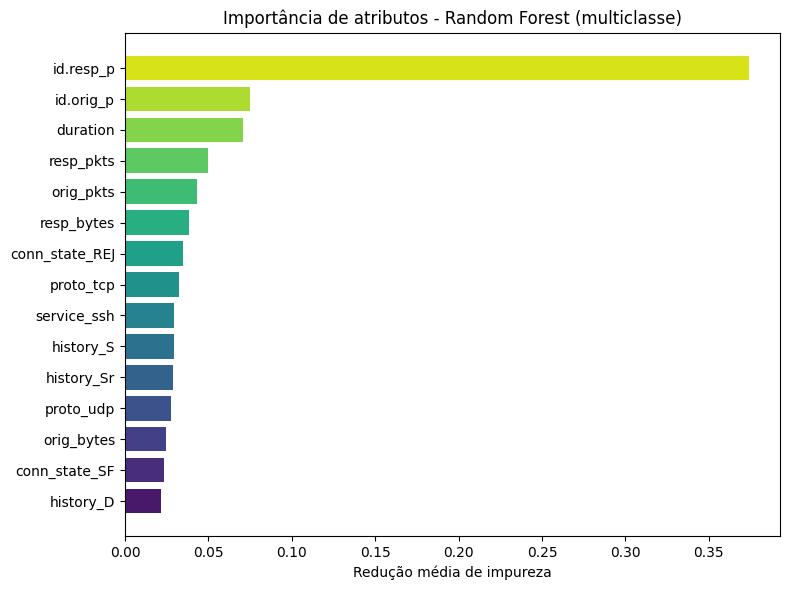
\includegraphics[width=0.75\textwidth]{figuras/importancia_atributos_rf_multiclasse.png}
\caption{Os 15 atributos mais importantes do Random Forest multiclasse (redução média de impureza).}
\label{fig:importancia}
\par\vspace{2pt}
\small{Fonte: elaborado pelo autor.}
\end{figure}

A Tabela~\ref{tab:portas-classe} mostra as portas de destino mais frequentes nas classes envolvidas nas principais confusões do SVM e da CNN. A classe DDoS utiliza a porta 80 em 99,4\% dos fluxos, enquanto o portscan se concentra nas portas 23, 22, 8080, 81 e 2323, associadas a serviços como Telnet e SSH, alvos comuns de varreduras em dispositivos IoT. Já o tráfego benigno é disperso, sem nenhuma porta acima de 3\% dos fluxos.

\begin{table}[htbp]
\centering
\caption{Portas de destino mais frequentes por classe no conjunto de treino (\% dos fluxos da classe).}
\label{tab:portas-classe}
\begin{tabular}{lll}
\toprule
\textbf{DDoS} & \textbf{Portscan} & \textbf{Benigno} \\
\midrule
80 (99,4\%)  & 23 (36,6\%)   & 81 (2,9\%) \\
5376 (0,6\%) & 22 (16,7\%)   & 123 (2,8\%) \\
             & 8080 (14,1\%) & 53 (2,1\%) \\
             & 81 (13,3\%)   & 22 (2,1\%) \\
             & 2323 (9,7\%)  & 1 (1,0\%) \\
\bottomrule
\end{tabular}
\\[2pt]
\small{Fonte: elaborado pelo autor.}
\end{table}

Esses dados ajudam a explicar o padrão de erros observado na Seção~\ref{sec:res-convencional}. Para uma árvore, separar DDoS de portscan exige uma única regra (por exemplo, ``porta de destino igual a 80''). Para SVM e CNN, que recebem a porta como um valor numérico padronizado, as portas 22, 23, 80 e 81 são valores muito próximos dentro de uma escala que vai até 65.535, e as classes que as utilizam ocupam praticamente a mesma região do espaço de atributos.

% ---------------------------------------------------------------------
\section{Avaliação com a distribuição natural das classes}
\label{sec:res-natural}

No conjunto de teste construído com a proporção natural das classes, nenhum fluxo de Okiru pôde ser incluído: todos os fluxos amostrados dessa classe correspondiam a padrões já presentes no treino. O mesmo ocorreu com quase todos os fluxos de DDoS, classe que ficou com uma única amostra. O conjunto resultante tem 10.272 fluxos, dos quais 9.952 (96,9\%) são de portscan e 297 são benignos. Nesse recorte, os modelos binários alcançaram F1-macro de 0,9966 (RF), 0,9940 (AD), 0,9905 (SVM) e 0,9710 (CNN). Esses valores confirmam o bom desempenho na detecção de portscan, mas não permitem conclusões sobre as demais classes. A principal constatação desse experimento é, portanto, outra: em proporção natural, o IoT-23 é dominado por poucos padrões de tráfego que se repetem milhões de vezes.

% ---------------------------------------------------------------------
\section{Generalização para cenários não vistos}
\label{sec:res-loso}

A Tabela~\ref{tab:loso-f1} apresenta o F1-macro da tarefa binária no protocolo LOSO (Seção~\ref{sec:loso}), em que cada captura maliciosa é retirada do treino e usada como teste. A Figura~\ref{fig:loso} mostra a taxa de detecção correspondente, isto é, a porcentagem dos fluxos maliciosos da captura retirada que cada modelo identificou.

\begin{table}[htbp]
\centering
\caption{F1-macro da tarefa binária no protocolo LOSO, por captura retirada do treino.}
\label{tab:loso-f1}
\begin{tabular}{lrrrr}
\toprule
\textbf{Captura retirada} & \textbf{RF} & \textbf{AD} & \textbf{SVM} & \textbf{CNN} \\
\midrule
Malware 1-1  & 0,6143 & 0,3016 & 0,6115 & 0,6136 \\
Malware 3-1  & 0,3670 & 0,4547 & 0,5300 & 0,8752 \\
Malware 8-1  & 0,3605 & 0,1306 & 0,9984 & 0,9980 \\
Malware 9-1  & 0,7360 & 0,7574 & 0,9868 & 0,9662 \\
Malware 34-1 & 0,6338 & 0,3650 & 0,7146 & 0,3546 \\
Malware 36-1 & 0,0807 & 0,0807 & 0,0807 & 0,0774 \\
\midrule
\textbf{Média}                      & 0,4654 & 0,3483 & \textbf{0,6537} & 0,6475 \\
\textbf{Teste convencional}         & 0,9983 & 0,9990 & 0,9554 & 0,9713 \\
\textbf{Queda}                      & $-$0,5329 & $-$0,6507 & $-$0,3017 & $-$0,3238 \\
\bottomrule
\end{tabular}
\\[2pt]
\small{Fonte: elaborado pelo autor.}
\end{table}

\begin{figure}[htbp]
\centering
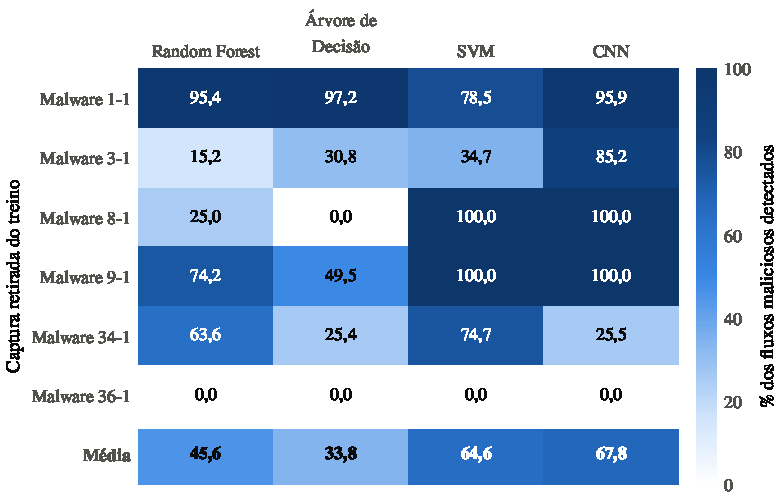
\includegraphics[width=0.78\textwidth]{figuras/loso_deteccao.pdf}
\caption{Taxa de detecção dos fluxos maliciosos da captura retirada do treino, por modelo, no protocolo LOSO.}
\label{fig:loso}
\par\vspace{2pt}
\small{Fonte: elaborado pelo autor.}
\end{figure}

Todos os modelos sofreram queda acentuada em relação ao protocolo convencional, mas a ordem entre eles se inverteu. As árvores, que lideravam o protocolo convencional, foram as que mais perderam desempenho: o F1-macro médio caiu para 0,47 no RF e 0,35 na AD, com taxas médias de detecção de 46\% e 34\%. SVM e CNN mantiveram F1-macro médio de 0,65, detectando em média 65\% e 68\% dos ataques inéditos. A diferença é mais nítida nas capturas 8-1 e 9-1. Na 8-1, SVM e CNN detectaram 100\% do tráfego de comando e controle do malware Hakai, contra 25\% do RF e nenhum fluxo da AD. Na 9-1, SVM e CNN detectaram toda a varredura de portas, contra 74\% do RF e 50\% da AD. O SVM superou ambas as árvores em F1-macro em quatro das seis capturas (3-1, 8-1, 9-1 e 34-1), e a CNN, em três.

Dois cenários merecem destaque. Na captura 36-1, nenhum dos modelos detectou um único fluxo malicioso: as classes Okiru e C\&C-HeartBeat existem apenas nessa captura, e, uma vez retiradas do treino, seu tráfego foi integralmente classificado como benigno. Na captura 1-1, por outro lado, as taxas de detecção foram altas (de 79\% a 97\%), mas acompanhadas de muitos falsos positivos nos fluxos benignos da própria captura: 25\% no SVM, 30\% no RF e na CNN e 76\% na AD. Esse resultado mostra que o tráfego benigno de dispositivos e redes não vistos no treino também é difícil de classificar. Considerando a média das seis capturas, a taxa de falsos positivos nos fluxos benignos do cenário retirado foi de 6,0\% no SVM, 7,3\% na CNN, 9,8\% no RF e 17,8\% na AD, Já nos fluxos benignos de \textit{honeypot}, cujo padrão está representado no treino, os falsos positivos foram nulos para RF e AD e de 0,6\% em média para o SVM. A CNN foi a exceção, com média de 4,7\%, concentrada em duas rodadas (12,4\% e 13,2\% nas capturas 34-1 e 36-1).

Na tarefa multiclasse, o F1-macro médio no LOSO foi de 0,17 (RF), 0,15 (AD) e 0,16 (CNN). Esse resultado é esperado: em cada rodada, ao menos parte do tráfego malicioso pertence a classes que nunca aparecem no treino ou que nele estão sub-representadas, e um classificador supervisionado não pode atribuir uma amostra a uma classe que não conhece. Por esse motivo, a análise de generalização concentrou-se na tarefa binária.

% ---------------------------------------------------------------------
\section{Efeito da representação das portas}
\label{sec:res-portas}

A Tabela~\ref{tab:portas-resumo} e a Figura~\ref{fig:portas} apresentam o resultado do experimento descrito na Seção~\ref{sec:exp-portas}, que alterou apenas a forma como as portas são apresentadas aos modelos.

\begin{table}[htbp]
\centering
\caption{Efeito da representação das portas no protocolo convencional e no LOSO.}
\label{tab:portas-resumo}
\small
\setlength{\tabcolsep}{4pt}
\begin{tabular}{llrrrr}
\toprule
 & & \multicolumn{2}{c}{\textbf{Convencional (F1-macro)}} & \multicolumn{2}{c}{\textbf{LOSO binário (média)}} \\
\cmidrule(lr){3-4} \cmidrule(lr){5-6}
\textbf{Modelo} & \textbf{Portas} & \textbf{Binária} & \textbf{Multiclasse} & \textbf{F1-macro} & \textbf{Detecção (\%)} \\
\midrule
RF  & numéricas    & 0,9983 & 0,9950 & 0,4654 & 45,6 \\
    & removidas    & 0,8286 & 0,4581 & 0,7800 & 83,8 \\
\midrule
AD  & numéricas    & 0,9990 & 0,9973 & 0,3483 & 33,8 \\
    & removidas    & 0,8281 & 0,4653 & 0,8499 & 91,9 \\
\midrule
CNN & numéricas    & 0,9713 & 0,7153 & 0,6475 & 67,8 \\
    & categóricas  & 0,9937 & 0,8059 & 0,3297 & 18,6 \\
\midrule
SVM & numéricas (referência) & 0,9554 & 0,7502 & 0,6537 & 64,7 \\
\bottomrule
\end{tabular}
\\[2pt]
\small{Fonte: elaborado pelo autor.}
\end{table}

\begin{figure}[htbp]
\centering
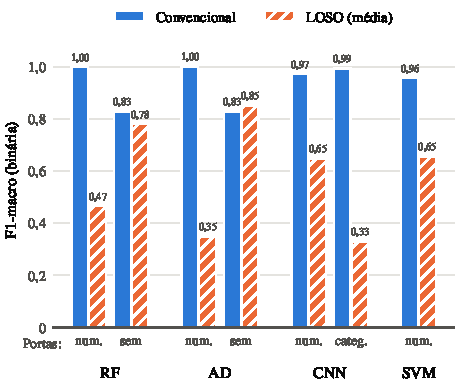
\includegraphics[width=\textwidth]{figuras/portas_normal_vs_loso.pdf}
\caption{F1-macro na tarefa binária no protocolo convencional e no LOSO, conforme a representação das portas.}
\label{fig:portas}
\par\vspace{2pt}
\small{Fonte: elaborado pelo autor.}
\end{figure}

A alteração produziu efeitos opostos nos dois grupos de modelos. Sem as portas, RF e AD perderam desempenho no protocolo convencional: o F1-macro caiu para 0,83 na tarefa binária e para menos de 0,47 na multiclasse, com queda do \textit{recall} da classe benigna para 0,76 (RF) e 0,73 (AD). Em contrapartida, sua capacidade de detectar ataques inéditos aumentou de forma expressiva: a taxa média de detecção no LOSO passou de 46\% para 84\% no RF e de 34\% para 92\% na AD, e o F1-macro médio da AD (0,85) superou o de todos os modelos originais. Na CNN, ocorreu o inverso. Com as portas codificadas como categorias, o desempenho no protocolo convencional melhorou (de 0,97 para 0,99 na binária e de 0,72 para 0,81 na multiclasse), com a precisão em portscan subindo de 0,65 para 0,99. Por outro lado, a taxa média de detecção no LOSO caiu de 68\% para 19\%.

A Tabela~\ref{tab:portas-loso} detalha a taxa de detecção por captura. O caso mais marcante é o da captura 36-1: o tráfego do Okiru, que nenhum modelo original detectava, passou a ser identificado em 96\% dos fluxos pelas duas árvores sem portas. Do mesmo modo, a AD sem portas detectou 100\% do tráfego da captura 8-1, que a AD original não detectava, e 98\% da captura 34-1, contra 25\% originalmente. Na CNN com portas categóricas, a detecção caiu a zero ou próximo de zero em quatro das seis capturas.

\begin{table}[htbp]
\centering
\caption{Taxa de detecção (\%) no LOSO binário, por captura, conforme a representação das portas.}
\label{tab:portas-loso}
\small
\begin{tabular}{lrrrrrr}
\toprule
 & \multicolumn{2}{c}{\textbf{RF}} & \multicolumn{2}{c}{\textbf{AD}} & \multicolumn{2}{c}{\textbf{CNN}} \\
\cmidrule(lr){2-3} \cmidrule(lr){4-5} \cmidrule(lr){6-7}
\textbf{Captura retirada} & \textbf{numéricas} & \textbf{sem} & \textbf{numéricas} & \textbf{sem} & \textbf{numéricas} & \textbf{categóricas} \\
\midrule
Malware 1-1  & 95,4 & 95,9  & 97,2 & 95,9  & 95,9  & 62,2 \\
Malware 3-1  & 15,2 & 22,9  & 30,8 & 60,8  & 85,2  &  0,0 \\
Malware 8-1  & 25,0 & 100,0 &  0,0 & 100,0 & 100,0 &  0,0 \\
Malware 9-1  & 74,2 & 100,0 & 49,5 & 100,0 & 100,0 & 49,5 \\
Malware 34-1 & 63,6 & 87,9  & 25,4 & 98,3  & 25,5  &  0,1 \\
Malware 36-1 &  0,0 & 96,3  &  0,0 & 96,4  &  0,0  &  0,0 \\
\midrule
\textbf{Média} & 45,6 & 83,8 & 33,8 & 91,9 & 67,8 & 18,6 \\
\bottomrule
\end{tabular}
\\[2pt]
\small{Fonte: elaborado pelo autor.}
\end{table}

O ganho de generalização das árvores sem portas não veio acompanhado de aumento relevante de falsos positivos no LOSO. Nos fluxos benignos das capturas retiradas, a taxa média de falsos positivos foi de 9,7\% no RF e 8,6\% na AD sem portas, valores próximos ou inferiores aos dos modelos originais (9,8\% e 17,8\%). A principal exceção continua sendo a captura 1-1, com cerca de 30\% de falsos positivos. O custo dessa representação aparece, portanto, no protocolo convencional, em que a queda do \textit{recall} benigno indica uma taxa de alarmes falsos incompatível com o uso prático.

Como RF e AD são determinísticos para uma mesma semente e um mesmo conjunto de dados, as diferenças observadas nesses modelos se devem exclusivamente à mudança na representação das portas. Para a CNN, os resultados do LOSO e do experimento das portas referem-se a uma única execução e estão sujeitos à variabilidade entre sementes observada na Seção~\ref{sec:res-ajuste}.
